\documentclass[border=5pt]{standalone}
\usepackage{tikz}
\usetikzlibrary{arrows.meta, calc}
\begin{document}
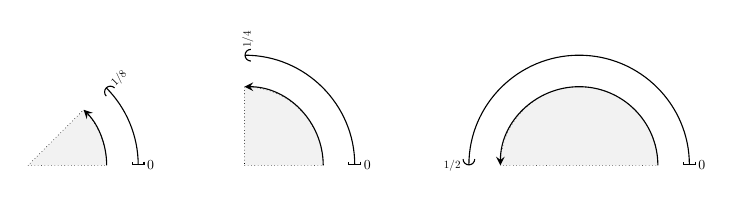
\begin{tikzpicture}
  \begin{scope}[xshift=-5cm]
    \filldraw[very thin, densely dotted, fill=gray!10!white] (0,0) -- (1,0) arc (0:45:1) -- (0,0);
    \draw[-stealth] (1,0) arc (0:45:1);

    \draw[{Bracket[]}-{Arc Barb[]}] (1.4,0) arc (0:45:1.4)
    node[scale=.5,  at start, right, xshift=3pt] {$0$} node[scale=.4,
    at end, sloped, xshift=3pt, yshift=3pt, rotate=90, right] {$1/8$};
  \end{scope}

  \begin{scope}[xshift=-2.25cm]
    \filldraw[very thin, densely dotted, fill=gray!10!white] (0,0) -- (1,0) arc (0:90:1) -- (0,0);
    \draw[-stealth] (1,0) arc (0:90:1);

    \draw[{Bracket[]}-{Arc Barb[]}] (1.4,0) arc (0:90:1.4)
    node[scale=.5,  at start, right, xshift=3pt] {$0$} node[scale=.4,
    at end, sloped, xshift=3pt, yshift=3pt, rotate=90, right] {$1/4$};
  \end{scope}

  \begin{scope}[xshift=2cm]
    \filldraw[very thin, densely dotted, fill=gray!10!white] (0,0) -- (1,0) arc (0:180:1) -- (0,0);
    \draw[-stealth] (1,0) arc (0:180:1);

    \draw[{Bracket[]}-{Arc Barb[]}] (1.4,0) arc (0:180:1.4)
    node[scale=.5,  at start, right, xshift=3pt] {$0$} node[scale=.4,
    at end, left, xshift=-4pt] {$1/2$};
  \end{scope}


\end{tikzpicture}
\end{document}
